\documentclass{InsightArticle}

\usepackage[dvips]{graphicx}
\usepackage{float}
\usepackage{subfigure}

\usepackage[dvips,
bookmarks,
bookmarksopen,
backref,
colorlinks,linkcolor={blue},citecolor={blue},urlcolor={blue},
]{hyperref}

\title{Criminisi Inpainting}

% 
% NOTE: This is the last number of the "handle" URL that 
% The Insight Journal assigns to your paper as part of the
% submission process. Please replace the number "1338" with
% the actual handle number that you get assigned.
%
\newcommand{\IJhandlerIDnumber}{3250}

% Increment the release number whenever significant changes are made.
% The author and/or editor can define 'significant' however they like.
\release{0.00}

% At minimum, give your name and an email address.  You can include a
% snail-mail address if you like.

\author{David Doria}
\authoraddress{Rensselaer Polytechnic Institute, Troy NY}


\begin{document}

\IJhandlefooter{\IJhandlerIDnumber}


\ifpdf
\else
   %
   % Commands for including Graphics when using latex
   % 
   \DeclareGraphicsExtensions{.eps,.jpg,.gif,.tiff,.bmp,.png}
   \DeclareGraphicsRule{.jpg}{eps}{.jpg.bb}{`convert #1 eps:-}
   \DeclareGraphicsRule{.gif}{eps}{.gif.bb}{`convert #1 eps:-}
   \DeclareGraphicsRule{.tiff}{eps}{.tiff.bb}{`convert #1 eps:-}
   \DeclareGraphicsRule{.bmp}{eps}{.bmp.bb}{`convert #1 eps:-}
   \DeclareGraphicsRule{.png}{eps}{.png.bb}{`convert #1 eps:-}
\fi


\maketitle


\ifhtml
\chapter*{Front Matter\label{front}}
\fi

\begin{abstract}
\noindent
This document presents a system to fill a hole in an image by copying patches from elsewhere in the image. These patches should be a good continuation of the hole boundary into the hole. The patch copying is done in an order which attempts to preserve linear structures in the image. This implementation is based on the algorithm described in ``Object Removal by Exemplar-Based Inpainting'' (Criminisi et. al.).

The code is available here:
https://github.com/daviddoria/Inpainting

\end{abstract}

\IJhandlenote{\IJhandlerIDnumber}

\tableofcontents
\section{Introduction}
This document presents a system to fill a hole in an image by copying patches from elsewhere in the image. These patches should be a good continuation of the hole boundary into the hole. The patch copying is done in an order which attempts to preserve linear structures in the image. This implementation is entirely based on the algorithm described in \cite{criminisi}. There are many subtle details of the implementation which are explained throughout this paper.

\section{Terminology}
Throughout this document, the ``source region'' is the portion of the image which is known (is not part of the hole) at the beginning. The ``target region'' is the current hole to be filled.

\section{Algorithm Overview}
The inputs to the algorithm consist of an image and a binary mask the same size as the image. Non-zero pixels in the mask indicate the region of the image which is to be considered the hole to inpaint/complete. Throughout this paper, we have colored the region in the input image corresponding to the hole bright green. This color irrelevant - we have done this only to make it obvious to tell if any part of the hole remains after inpainting (it should not). In practice, the input image need not be modified.

\section{Algorithm Synthetic Demonstration}
Figure \ref{fig:SyntheticDemonstration} shows a synthetic demonstration of the algorithm. The image consists of a black region (top) and a gray region (bottom).  This simple example is used for testing because we know the result to expect - the dividing line between the black region and gray region should be continued smoothly.

\begin{figure}[H]
\centering
\subfigure[Image to be filled. The region to be filled is shown in bright green.]
  {
  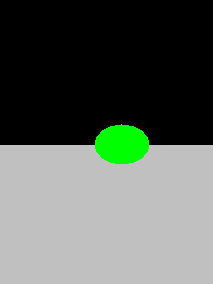
\includegraphics[width=0.3\linewidth]{images/BlackWhite}
  \label{fig:SyntheticDemonstration:ExampleInputImage}
  }
\subfigure[The mask of the region to inpaint.]
  {
  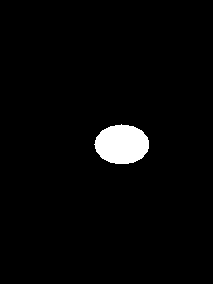
\includegraphics[width=0.3\linewidth]{images/BlackWhiteMask}
  \label{fig:SyntheticDemonstration:ExampleInputMask}
  }
\subfigure[The result of the inpainting.]
  {
  
\includegraphics[width=0.3\linewidth]{images/BlackWhiteResult}
  \label{fig:SyntheticDemonstration:ExampleInputOutput}
  }
\caption{Synthetic Demonstration}
\label{fig:SyntheticDemonstration}
\end{figure}

\section{Algorithm Realistic Demonstration}
Figure \ref{fig:RealisticDemonstration} shows a real example of the algorithm. This result shows the typical quality of inpainting that the algorithm produces. 

\begin{figure}[H]
\centering
\subfigure[Image to be filled. The region to be filled is shown in bright green.]
  {
  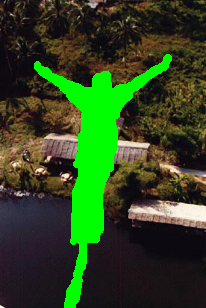
\includegraphics[width=0.3\linewidth]{images/Bungee}
  \label{fig:RealisticDemonstration:ExampleInputImage}
  }
\subfigure[The mask of the region to inpaint.]
  {
  
\includegraphics[width=0.3\linewidth]{images/BungeeMask}
  \label{fig:RealisticDemonstration:ExampleInputMask}
  }
\subfigure[The result of the inpainting. This took about 30 seconds on a P4 3GHz processor with a 206x308 image and a patch radius = 5.]
  {
  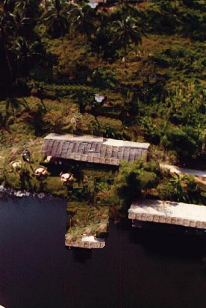
\includegraphics[width=0.3\linewidth]{images/BungeeResult}
  \label{fig:RealisticDemonstration:ExampleInputOutput}
  }
\caption{Realistic Demonstration}
\label{fig:RealisticDemonstration}
\end{figure}

\section{Algorithm Structure}
An overview of the algorithm is:
\begin{itemize}
  \item Initialize:
    \begin{itemize}
      \item Read an image and a binary mask. Non-zero pixels in the mask describe the hole to fill.
      \item Set the size of the patches which will be copied. (Typically an 11x11 patch (patch radius = 5) is used).
      \item Locate all patches of the image which are completely inside the image and completely in the source region. These are stored as an $std::vector<itk::ImageRegion<2> >$ named SourcePatches.
    \end{itemize}

  \item Main loop:
  \begin{itemize}
    \item Compute the priority of every pixel on the hole boundary (see Section \ref{subsec:AlgorithmDetails:Priorities})
    \item Determine the boundary pixel with the highest priority. We will call this the target pixel. The region centered at the target pixel and the size of the patches is called the target patch.
    \item Find the SourcePatch which best matches the portion of the target patch in the source region.
    \item Copy the corresponding portion of the source patch into the target region of the target patch.
    \item Repeat until the target region consists of zero pixels.
  \end{itemize}
\end{itemize}

%%%%%%%%%%%%%%%
\section{Algorithm Details}
\label{sec:AlgorithmDetails}

The two main parts of the algorithm are
\begin{enumerate}
 \item Determine the priority of each boundary pixel. This determines the order with which the hole is filled.
 \item Find the best matching patch to the patch around the pixel with the highest priority.
\end{enumerate}


\subsection{Priorities}
\label{subsec:AlgorithmDetails:Priorities}

The priority $P(p)$ of a pixel $p$ is given by the product of a Confidence term $C(p)$ and a Data term $D(p)$.
\begin{equation}
P(p) = C(p)D(p)
\end{equation}

The original author describes the terms:

``C(p) may be thought of as a measure of the amount of reliable information surrounding the pixel 'p'. The intention is to fill first those patches which have more of their pixels already filled, with additional preference given to pixels that were filled early on (or that were never part of the target region).''

``D(p) is a function of the strength of the isophotes hitting the front at each iteration. This term boosts the priority of a patch that an isophot ''flows`` into. This factor is of fundamental importance in our algorithm because it encourages linear structures to be synthesized first, and, therefore propagated securely into the target region.''

\subsubsection{Confidence Term}
The confidence term is computed as:
\begin{equation}
 C(p) = \frac{\sum \mbox{Confidences of patch pixels in the source region}}{\mbox{Area of the patch}}
\end{equation}

To initialize, the confidence inside the hole is set to $0$ and the confidence outside the hole is set to $1$.

\subsubsection{Data Term}
The data term is computed as:
\begin{equation}
 D(p) = \frac{\mbox{dot}(\mbox{isophote}, \mbox{boundary normal})}{\alpha}
\end{equation}

$\alpha$ is a normalization factor that should be set to $255$ for grayscale images, but that value also seems to work well for RGB images.

No initialization is necessary because this term is not recursive - it can be computed from the data directly at each iteration.

\subsection{Patch Matching}
\label{subsec:AlgorithmDetails:PatchMatching}
To compare two patches (a source patch and a target patch), we compute the normalized sum of squared differences between every pixel which is in the source region of target patches (all pixels of the SourcePatch are in the source region by definition).

%%%%%%%%%%%%%%%
\section{Implementation Details}
\label{sec:ImplementationDetails}

\subsection{Isophotes}
An isophotes is simply a gradient vector rotated by 90 degrees. It indicates the direction of ``same-ness'' rather than the direction of maximum difference. There is a small trick, however, to computing the isophotes. We originally tried to compute the isophotes using the following procedure:

\begin{itemize}
 \item Convert the RGB image to a grayscale image.
 \item Blur the grayscale image.
 \item Compute the gradient using itkGradientImageFilter.
 \item Rotate the resulting vectors by 90 degrees.
 \item Keep only the values in the source region.
\end{itemize}

This procedure produces the gradient magnitude map shown in Figure \ref{fig:ErroneousGradient}.
\begin{figure}[H]
  \centering
  
\includegraphics[width=0.3\linewidth]{images/ErroneousGradient}
  \caption{Result of naively computing the image gradient.}
  \label{fig:ErroneousGradient}
\end{figure}

The high values of the gradient magnitude surrounding the target region are very troublesome. The resulting gradient magnitude image using this technique is sensitive to the choice of the pixel values in the target region, which we actually want to be a completely arbitrary choice (it should not affect anything). More importantly, the gradient plays a large part in the computation of the pixel priorities, and this computation is greatly disturbed by these erroneous values. Simply ignoring these boundary isophotes is not an option because the isophotes on the boundary are exactly the ones that are used in the computation of the Data term. To fix this problem, we immediately dilate the mask specified by the user. This allows us to compute the isophotes as described above, but now we have image information on both sides of the hole boundary, leading to a valid gradient everywhere we need it to be. Figure \ref{fig:ErrorneousGradientCorrection} shows the procedure for fixing this problem.

\begin{figure}[H]
\centering
\subfigure[Image to be filled. The target region is shown in green.]
  {
  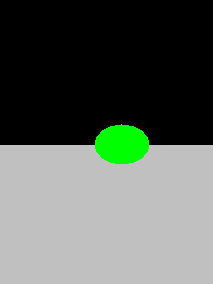
\includegraphics[width=0.3\linewidth]{images/BlackWhite}
  \label{fig:ErrorneousGradientCorrection:InputImage}
  }
\subfigure[The dilated mask.]
  {
  
\includegraphics[width=0.3\linewidth]{images/BlackWhiteDilatedMask}
  \label{fig:ErrorneousGradientCorrection:InputDilated}
  }
\subfigure[The gradient magnitude with pixels in the new (enlarged) target region set to zero.]
  {
  
\includegraphics[width=0.3\linewidth]{images/MaskedGradientMagnitude}
  \label{fig:ErrorneousGradientCorrection:Output}
  }
\caption{Procedure for fixing the erroneous gradient problem.}
\label{fig:ErrorneousGradientCorrection}
\end{figure}

As you can see, this gradient magnitude image is exactly what we would expect.

\subsection{Boundary Normals}
There are two things to be careful with when computing the boundary normals: computing the normals only on the one pixel thick boundary, and using the correct side of the masked region as the boundary.

\subsubsection{Computing boundary normals only on the one pixel thick boundary}
If we compute the normals directly on the binary mask, the set of resulting vectors are too discretized to be of use. Therefore, we first blur the mask. However, the gradient of the blurred mask results in non-zero vectors in the gradient image in many more pixels (a ``thick'' boundary) than the gradient of the original mask (a single pixel ``thin'' boundary). Therefore, we must mask the gradient of the blurred mask to keep only the pixels which would have been non-zero in the original mask gradient.


\subsubsection{Using the correct side of the masked region as the boundary}
There are two potential boundaries that can be extracted from a masked region - the ``inner'' boundary and the ``outer'' boundary. As shown in Figure \ref{fig:BoundarySide}, the inner boundary (red) is composed of pixels originally on the white (masked) side of the blob, and the outer boundary (green) is composed of pixels originally on the black (unmasked) side of the blob. It is important that we use the outer boundary, because we need the boundary to be defined at the same pixels that we have image information, which is only in the source (black/unmasked) region.

\begin{figure}[H]
\centering
\subfigure[The inner boundary.]
  {
  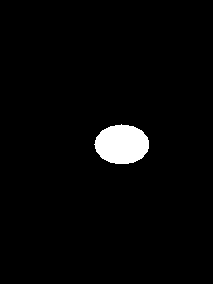
\includegraphics[width=0.3\linewidth]{images/BlackWhiteMask}
  \label{fig:BoundarySide:Mask}
  }
\subfigure[Outer boundary (green) and inner boundary (red).]
  {
  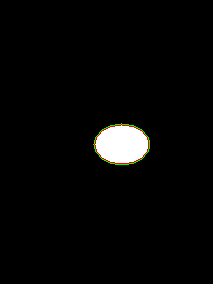
\includegraphics[width=0.3\linewidth]{images/BothBoundaries}
  \label{fig:BoundarySide:BothBoundaries}
  }
\caption{Inner vs Outer Boundary of a Region}
\label{fig:BoundarySide}
\end{figure}

\subsubsection{Code Snippet}
The CriminisiInpainting class must be instantiated using the type of image to be inpainted. Then the patch radius must be set, the image and mask provided, and the Inpaint() function called.
\begin{verbatim}
  CriminisiInpainting<ImageType> Inpainting;
  Inpainting.SetPatchRadius(5);
  Inpainting.SetImage(imageReader->GetOutput());
  Inpainting.SetInputMask(maskReader->GetOutput());
  Inpainting.Inpaint();

  ImageType::Pointer result = Inpainting.GetResult();

\end{verbatim}

If you would like to see what happens at every step of the algorithm, you can use:
\begin{verbatim}
Inpainting.SetWriteIntermediateImages(true); 
\end{verbatim}
NOTE: Several images are output at each iteration - these files could be quite large!


%%%%%%%%%%%%%%%
\begin{thebibliography}{9}

	\bibitem{criminisi}
	  A. Criminisi, P. Perez, K. Toyama,
	  \emph{Object Removal by Exemplar-Based Inpainting}.
	  Computer Vision and Pattern Recognition 2003

\end{thebibliography}

\end{document}